\documentclass[11pt,openany]{book}
\usepackage[]{graphicx}\usepackage[]{color}
%% maxwidth is the original width if it is less than linewidth
%% otherwise use linewidth (to make sure the graphics do not exceed the margin)
\makeatletter
\def\maxwidth{ %
  \ifdim\Gin@nat@width>\linewidth
    \linewidth
  \else
    \Gin@nat@width
  \fi
}
\makeatother

\definecolor{fgcolor}{rgb}{0.345, 0.345, 0.345}
\newcommand{\hlnum}[1]{\textcolor[rgb]{0.686,0.059,0.569}{#1}}%
\newcommand{\hlstr}[1]{\textcolor[rgb]{0.192,0.494,0.8}{#1}}%
\newcommand{\hlcom}[1]{\textcolor[rgb]{0.678,0.584,0.686}{\textit{#1}}}%
\newcommand{\hlopt}[1]{\textcolor[rgb]{0,0,0}{#1}}%
\newcommand{\hlstd}[1]{\textcolor[rgb]{0.345,0.345,0.345}{#1}}%
\newcommand{\hlkwa}[1]{\textcolor[rgb]{0.161,0.373,0.58}{\textbf{#1}}}%
\newcommand{\hlkwb}[1]{\textcolor[rgb]{0.69,0.353,0.396}{#1}}%
\newcommand{\hlkwc}[1]{\textcolor[rgb]{0.333,0.667,0.333}{#1}}%
\newcommand{\hlkwd}[1]{\textcolor[rgb]{0.737,0.353,0.396}{\textbf{#1}}}%
\let\hlipl\hlkwb

\usepackage{framed}
\makeatletter
\newenvironment{kframe}{%
 \def\at@end@of@kframe{}%
 \ifinner\ifhmode%
  \def\at@end@of@kframe{\end{minipage}}%
  \begin{minipage}{\columnwidth}%
 \fi\fi%
 \def\FrameCommand##1{\hskip\@totalleftmargin \hskip-\fboxsep
 \colorbox{shadecolor}{##1}\hskip-\fboxsep
     % There is no \\@totalrightmargin, so:
     \hskip-\linewidth \hskip-\@totalleftmargin \hskip\columnwidth}%
 \MakeFramed {\advance\hsize-\width
   \@totalleftmargin\z@ \linewidth\hsize
   \@setminipage}}%
 {\par\unskip\endMakeFramed%
 \at@end@of@kframe}
\makeatother

\definecolor{shadecolor}{rgb}{.97, .97, .97}
\definecolor{messagecolor}{rgb}{0, 0, 0}
\definecolor{warningcolor}{rgb}{1, 0, 1}
\definecolor{errorcolor}{rgb}{1, 0, 0}
\newenvironment{knitrout}{}{} % an empty environment to be redefined in TeX

\usepackage{alltt}
\newcommand{\SweaveOpts}[1]{}  % do not interfere with LaTeX
\newcommand{\SweaveInput}[1]{} % because they are not real TeX commands
\newcommand{\Sexpr}[1]{}       % will only be parsed by R


\usepackage[utf8]{inputenc} 
\usepackage{amssymb, amsmath, amsthm}
\usepackage{fullpage}
\usepackage{setspace}
\usepackage{graphicx}
\usepackage{natbib}
\usepackage{rotating}
\usepackage{caption}
\usepackage{subcaption}
\usepackage{multirow}
\usepackage{booktabs}
\usepackage{dcolumn}
\usepackage[grey]{quotchap}
\usepackage{xcolor}
\usepackage[left=1in, top=1in, right=1.5in, bottom=1in, headsep=.5in]
{geometry}
\usepackage{fancyhdr, blindtext}
\usepackage{diagbox}
\usepackage{hyperref} 
\usepackage{placeins}
\renewenvironment{knitrout}{\begin{singlespace}}{\end{singlespace}}
\newcommand*{\mybox}[2]{\colorbox{#1!30}{\parbox{.98\linewidth}{#2}}}
\newcommand*{\befehl}[1]{\texttt{\textbackslash #1}} % Added by 


\fancyhf{}
\fancyhead[LE]{\slshape \rightmark} 
\fancyhead[RE]{\thepage}
\fancyhead[RO]{\slshape \leftmark} 
\fancyhead[LO]{\thepage}
\renewcommand{\headrulewidth}{0.4pt}
\pagestyle{fancy}
%% new command for greybox
\long\def\greybox#1{%
    \newbox\contentbox%
    \newbox\bkgdbox%
    \setbox\contentbox\hbox to \hsize{%
        \vtop{
            \kern\columnsep
            \hbox to \hsize{%
                \kern\columnsep%
                \advance\hsize by -2\columnsep%
                \setlength{\textwidth}{\hsize}%
                \vbox{
                    \parskip=\baselineskip
                    \parindent=0bp
                    #1
                }%
                \kern\columnsep%
            }%
            \kern\columnsep%
        }%
    }%
    \setbox\bkgdbox\vbox{
        \pdfliteral{0.85 0.85 0.85 rg}
        \hrule width  \wd\contentbox %
               height \ht\contentbox %
               depth  \dp\contentbox
        \pdfliteral{0 0 0 rg}
    }%
    \wd\bkgdbox=0bp%
    \vbox{\hbox to \hsize{\box\bkgdbox\box\contentbox}}%
    \vskip\baselineskip%
}
%% make greybox (grbox) a float
\usepackage{float}
\newfloat{grbox}{thp}{lop}[section]
\floatname{grbox}{Grey Box}



\begin{document}


\chapter{Inference}



This chapter considers the role of inference---learning about populations from samples---and the practical and theoretical importance of understanding the characteristics of your data before attempting to undertake statistical analysis. As we noted in the prior chapters, it is a vital first step in empirical analysis to ``roll in the data."

\section{Inference: Populations and Samples}

The basis of hypothesis testing with statistical analysis is \textbf{inference}. In short, inference---and inferential statistics by extension---means deriving knowledge about a population from a sample of that population. Given that in most contexts it is not possible to have all the data on an entire population of interest, we therefore need to sample from that population.\footnote{It is important to keep in mind that, for purposes of theory building, the population of interest may not be finite. For example, if you theorize about general properties of human behavior, many of the members of the human population are not yet (or are no longer) alive. Hence it is not possible to include all of the population of interest in your research. We therefore rely on samples.} However, in order to be able to rely on inference, the sample must cover the theoretically relevant variables, variable ranges, and contexts. 

\subsection{Populations and Samples} 

In doing statistical analysis we differentiate between populations and samples.  The population is the total set of items that we care about.  The sample is a subset of those items that we study in order to understand the population.  While we are interested in the population we often need to resort to studying a sample due to time, financial, or logistic constraints that might make studying the entire population infeasible. Instead, we use inferential statistics to make inferences about the population from a sample.

\subsection{Sampling and Knowing} 

Take a relatively common -- but perhaps less commonly examined -- expression about what we ``know" about the world around us. We commonly say we ``know" people, and some we know better than others. What does it mean to know someone? In part it must mean that we can anticipate how that person would behave in a wide array of situations. If we know that person from experience, then it must be that we have observed their behavior across a 
sufficient variety of situations in the past to be able to infer how they would behave in  future situations. Put differently, we have ``sampled" their behavior across a relevant range of situations and contexts to be confident that we can anticipate their behavior in the future.\footnote{Of course, we also need to estimate changes -- both gradual and abrupt -- in how people behave over time, which is the province of time-series analysis.} Similar considerations about sampling might apply to ``knowing" a place, a group, or an institution. Of equal importance, samples of observations
across different combinations of variables are necessary to identify relationships (or functions) between variables.  In short, samples -- whether deliberately drawn and systematic or otherwise -- are integral to what we think we know of the world around us.

\subsection{Sampling Strategies} 

Given the importance of sampling, it should come as little surprise that there are numerous strategies designed to provide useful inference about populations. For example, how can we judge whether the temperature of a soup is appropriate before serving it? We might stir the pot, to assure uniformity of temperature across possible (spoon-sized) samples, then sample a spoonful. A particularly thorny problem in sampling concerns the practice of courtship, in which participants may attempt to put ``their best foot forward" to make a good impression. Put differently, the participants often seek to bias the sample of relational experiences to make themselves look better than they might on average. Sampling in this context usually involves (a) getting opinions of others, thereby broadening (if only indirectly) the size of the sample, and (b) observing the courtship partner over a wide range of circumstances in which the intended bias may be difficult to maintain. Put formally, we may try to stratify the sample by taking observations in appropriate ``cells" that correspond to different potential influences on behavior -- say, high stress environments involving preparation for final exams or meeting parents. In the best possible case, however, we try to wash out the effect of various influences on our samples through randomization. To pursue the courtship example (perhaps a bit too far!), observations of behavior could be taken across interactions from a randomly assigned array of partners and situations. But, of course, by then all bets are off on things working out anyway.

\subsection{Sampling Techniques}

When engaging in inferential statistics to infer about the characteristics a population from a sample, it is essential to be clear about how the sample was drawn. Sampling can be a very complex subject with multiple stages involved in drawing the final sample. It is desirable that the sample is some form of a \textbf{probability sample}, i.e., a sample in which each member of the population has a known probability of being sampled.   The most direct form of an appropriate probability sample is a \textbf{random sample} where everyone has the same probability of being sampled.  A random sample has the advantages of simplicity (in theory) and ease of inference as no adjustments to the data are needed.  But, the reality of conducting a random sample may make the process quite challenging.  Before we can draw subjects at random, we need a list of all members of the population.  For many populations (e.g. adult US residents) that list is impossible to get.  Not too long ago, it was reasonable to conclude that a list of telephone numbers was a reasonable approximation of such a listing for American households.  During the era that landlines were ubiquitous, pollsters could randomly call numbers (and perhaps ask for the adult in the household who had the most recent birthday) to get a good approximation of a national random sample.  (It was also an era before caller identification and specialized ringtones which meant that calls were routinely answered decreasing - but not eliminating - the concern with response bias.)  Of course, telephone habits have changed and pollsters finding it increasingly difficult to make the case that random dialing of landlines serves as a representative sample of adult Americans.

Other forms of probability sampling are frequently used to overcome some of the difficulties that pure random sampling presents.  Suppose our analysis will call upon us to make comparisons based on race.  Only 12.6\% of Americans are African-American.  Suppose we also want to take into account religious preference.  Only 5\% of African-Americans are Catholic, which means that only .6\% of the population is both.  If our sample size is 500, we might end up with three Catholic African-Americans.  A \textbf{stratified random sample} (also called a quota sample) can address that problem.  A stratified random sample is similar to a simple random sample, but will draw from different subpopulations, strata, at different rates.  The total sample needs to be weighted, then, to be representative of the entire population.
  
Another type of probability sample that is common in face-to-face surveys relies on \textbf{cluster sampling}.  Cluster sampling initially samples based on clusters (generally geographic units, such as census tracts) and then samples participants within those units.  In fact, this approach often uses multi-level sampling where the first level might be a sample of congressional districts, then census tracts, and then households.  The final sample will need to be weighted in a complex way to reflect varying probabilities that individuals will be included in the sample.  
  
\textbf{Non-probability samples}, or those for which the probability of inclusion of a member of the population in the sample is unknown, can raise difficult issues for statistical inference; however, under some conditions, they can be considered representative and used for inferential statistics.

\textbf{Convenience samples} (e.g., undergraduate students in the Psychology Department subject pool) are accessible and relatively low cost, but may differ from the larger population to which you want to infer in important respects.   Necessity may push a researcher to use a convenience sample, but inference should be approached with caution.  A convenience sample based on ``I asked people who come out of the bank" might provide quite different results from a sample based on ``I asked people who come out of a payday loan establishment".

Some non-probability samples are used because the researcher does not want to make inferences to a larger population.  A \textbf{purposive or judgmental sample} relies on the researcher's discretion regarding who can bring useful information to bear on the subject matter.  If we want to know why a piece of legislation was enacted, it makes sense to sample the author and co-authors of the bill, committee members, leadership, etc. rather than a random sample of members of the legislative body.

\textbf{Snowball sampling} is similar to a purposive sample in that we look for people with certain characteristics but rely on subjects to recommend others who meet the criteria we have in place.  We might want to know about struggling young artists.  They may be hard to find, though, since their works are not hanging in galleries so we may start with a one or more that we can find and then ask them who else we should interview.
	
Increasingly, various kinds of non-probability samples are employed in social science research, and when this is done it is critical that the potential biases associated with the samples be evaluated.  But there is also growing evidence that non-probability samples can be used inferentially - when done very carefully, using complex adjustments.  Wang, et al. (2014) demonstrate that a sample of Xbox users could be used to forecast the 2012 presidential election outcome. \footnote{Wei Wang, David Rothschild, Sharad Goel, and Andrew Gelman (2014)  ''Forecasting Elections with Non-Representative Polls," Preprint submitted to \textit{International Journal of Forecasting} March 31, 2014.}  The overview of the technique is relatively simple, but the execution is more challenging.  They divided their data into cells based on politically and demographically relevant variables (e.g., party id, gender, race, etc.) and ended up with over 175,000 cells - poststratification.  (There were about three-quarters of a million participants in the Xbox survey).  Basically, they found the vote intention within each cell and then weighted each cell based on a national survey using multilevel regression.   Their final results were strikingly accurate.   Similarly, Nate Silver with FiveThirtyEight, has demonstrated remarkable ability to forecast based on his weighted sample of polls taken by others.
  
Sampling techniques can be relatively straightforward, but as one moves away from simple random sampling, the sampling process either becomes more complex or limits our ability to draw inferences about a population.  Researchers use all of these techniques for good purposes and the best technique will depend on a variety of factors, such as budget, expertise, need for precision, and what research question is being addressed. For the remainder of this text, though, when we talk about drawing inferences, the data will based upon an appropriately drawn, probability sample.

%%%This is from the first edition for reference.
\subsection{So How is it That We Know?} 

So why is it that the characteristics of samples can tell us a lot about the characteristics of populations? If samples are properly drawn, the observations taken will provide a range of values on the measures of interest that reflect those of the larger population. The connection is that we expect the phenomenon we are measuring will have a \textbf{distribution} within the population, and a sample of observations drawn from the population will provide useful information about that distribution. The theoretical connection comes from probability theory, which concerns the analysis of random phenomena. For present purposes, if we randomly draw a sample of observations on a measure for an individual (say, discrete acts of kindness), we can use probability theory to make inferences about the characteristics of the overall population of the phenomenon in question. More specifically, probability theory allows us to make inference about the shape of that distribution -- how frequent are acts of kindness committed, or what proportion of acts evidence kindness?

In sum, samples provide information about  \textbf{probability distributions}. Probability distributions include all possible values and the probabilities associated with those values. The \textbf{normal distribution} is the key probability distribution in inferential statistics.

\section{The Normal Distribution} 

For purposes of statistical inference, the normal distribution is one of the most important types of probability distributions. It forms the basis of many of the assumptions needed to do quantitative data analysis, and is the basis for a wide range of hypothesis tests.  A standardized normal distribution has a mean, $\mu$, of $0$ and a standard deviation (s.d.), $\sigma$, of $1$. The distribution of an outcome variable, $Y$, can be
described: 

\begin{equation}
  \label{eq:norm}
  Y \sim N(\mu_Y,\sigma^{2}_Y)
\end{equation}

\noindent where $\sim$ stands for ``distributed as'', $N$ indicates the normal distribution, and mean $\mu_Y$ and variance $\sigma^{2}_Y$ are
the parameters. The probability function of the normal distribution is expressed below:

\begin{description}
  \item [The Normal Probability Density Function] The probability density function (PDF) of a normal
    distribution with mean $\mu$ and 
      standard deviation $\sigma$: 
      \begin{center}
        $f(x) = \frac{1}{\sigma \sqrt{2 \pi}} e^{-(x-\mu)^{2}/2\sigma^{2}}$
      \end{center}
  \item [The Standard Normal Probability Density Function] The
    standard normal PDF has a $\mu=0$ and $\sigma=1$
      \begin{center}
        $f(x) = \frac{1}{\sqrt{2 \pi}}e^{-x^{2}/2}$
      \end{center}     
\end{description}
Using the standard normal PDF, we can plot a normal distribution in
\texttt{R}.  
\begin{knitrout}
\definecolor{shadecolor}{rgb}{0.969, 0.969, 0.969}\color{fgcolor}\begin{kframe}
\begin{alltt}
\hlstd{x} \hlkwb{<-} \hlkwd{seq}\hlstd{(}\hlopt{-}\hlnum{4}\hlstd{,}\hlnum{4}\hlstd{,}\hlkwc{length}\hlstd{=}\hlnum{200}\hlstd{)}
\hlstd{y} \hlkwb{<-} \hlnum{1}\hlopt{/}\hlkwd{sqrt}\hlstd{(}\hlnum{2}\hlopt{*}\hlstd{pi)}\hlopt{*}\hlkwd{exp}\hlstd{(}\hlopt{-}\hlstd{x}\hlopt{^}\hlnum{2}\hlopt{/}\hlnum{2}\hlstd{)}
\hlkwd{plot}\hlstd{(x,y,} \hlkwc{type}\hlstd{=}\hlstr{"l"}\hlstd{,} \hlkwc{lwd}\hlstd{=}\hlnum{2}\hlstd{)}
\end{alltt}
\end{kframe}
\end{knitrout}
\begin{figure}
  \centering
  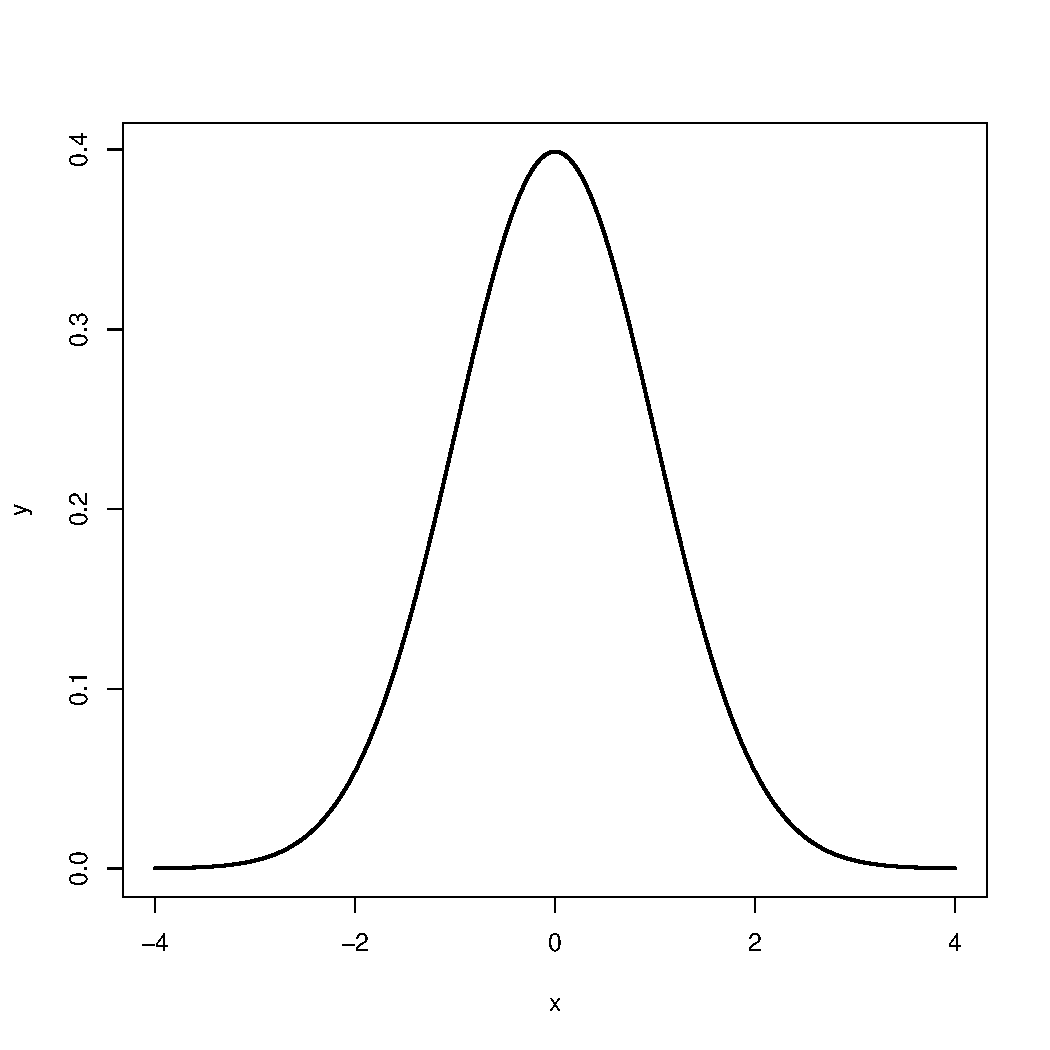
\includegraphics[width=4in]{../05_Inference/normal.pdf}% picture filename
  \caption[Normal Distribution]{The Normal Distribution  \label{normal}}
\end{figure}
\noindent Note that the the tails go to $\pm \infty$. In addition, the density of a distribution over the range of x is the key to hypothesis testing With a normal distribution, $\sim68\%$ of the observations will fall within $1$ standard deviation of the mean, $\sim 95\%$ will fall within 2 standard deviations, and $\sim 99.7\%$ within 3 standard deviations. This is illustrated in Figure \ref{fig:norm}. 





\begin{figure}
        \centering
        \begin{subfigure}[b]{0.4\textwidth}
                \centering
                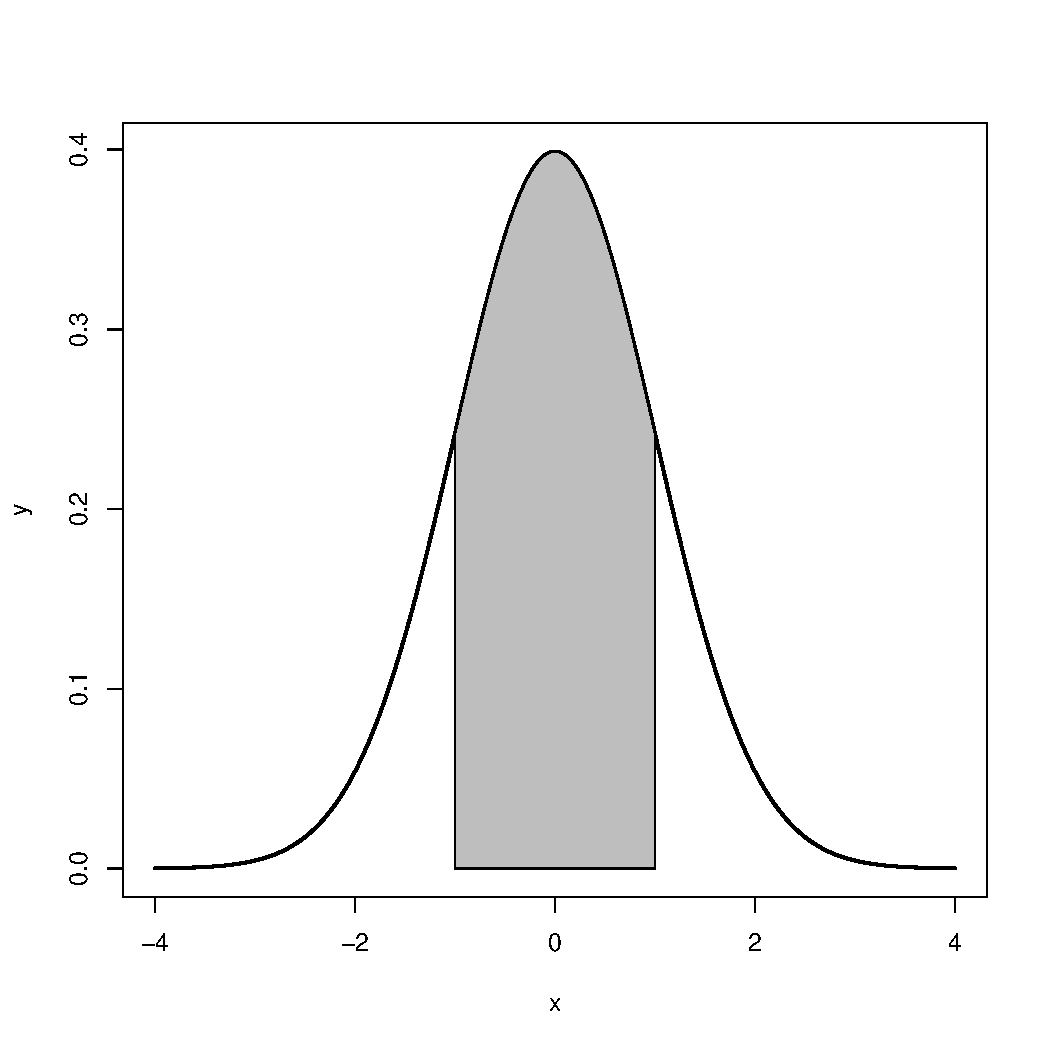
\includegraphics[width=\textwidth]{../05_Inference/normal68.pdf}
                \caption{$\sim 68\%$: 1 s.d. \label{fig:norm68}}
        \end{subfigure}
        \begin{subfigure}[b]{0.4\textwidth}
                \centering
                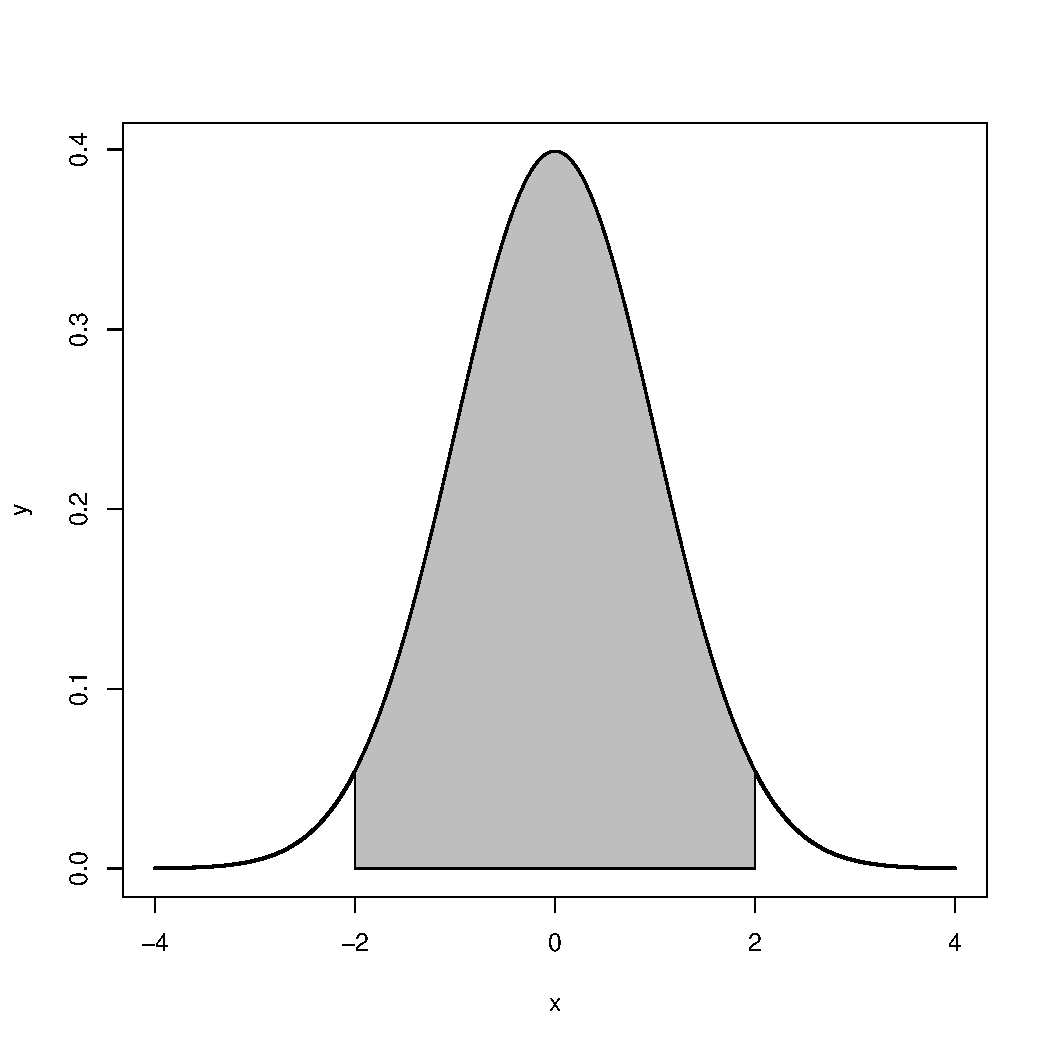
\includegraphics[width=\textwidth]{../05_Inference/normal95.pdf}
                \caption{$\sim 95\%$: 2 s.d.  \label{fig:norm95}}
        \end{subfigure}
        \begin{subfigure}[b]{0.4\textwidth}
                \centering
                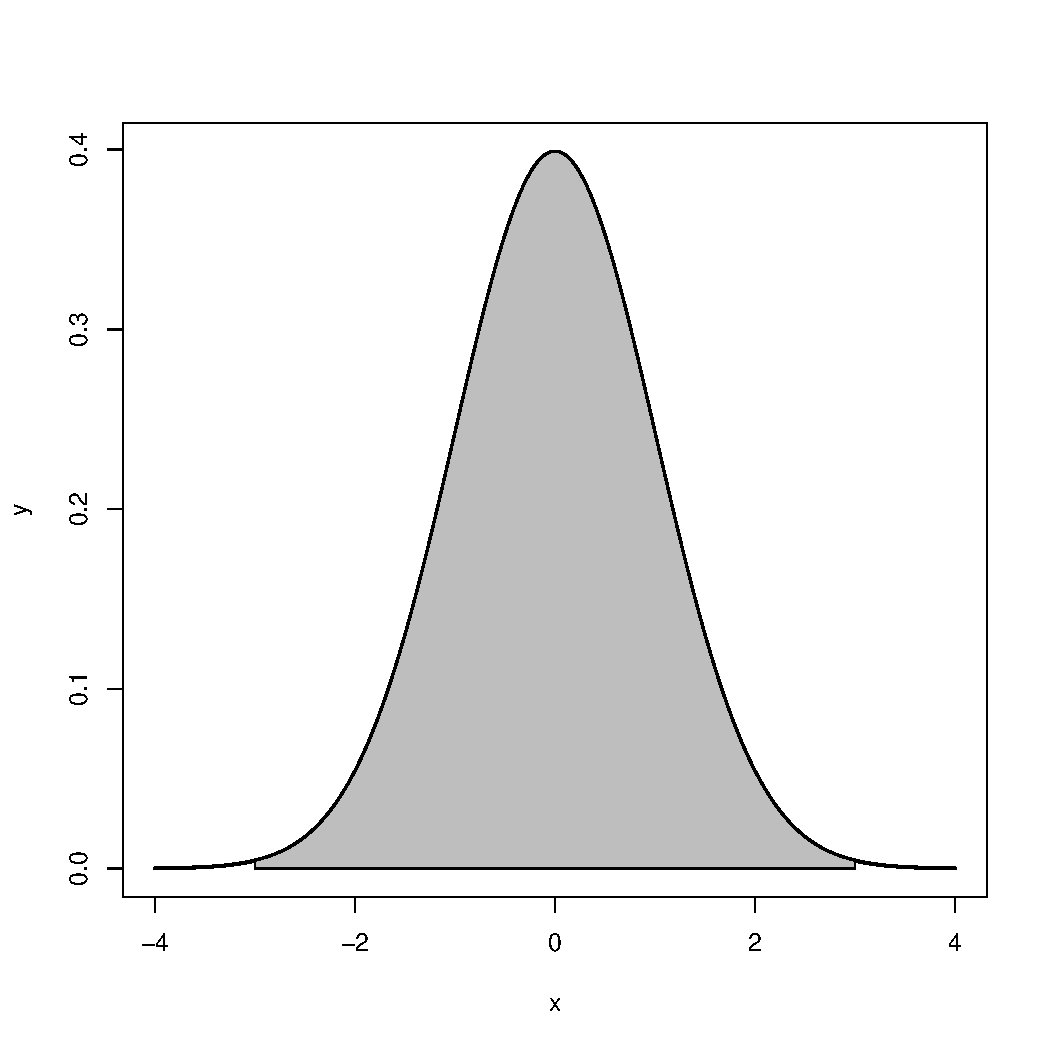
\includegraphics[width=\textwidth]{../05_Inference/normal99.pdf}
                \caption{$\sim 99.7\%$: 3 s.d. \label{fig:norm99}}
        \end{subfigure}
        \caption{Normal Distribution and Standard Deviations \label{fig:norm}}
\end{figure}

The normal distribution is characterized by several important properties. The distribution of observations is symmetrical around the mean $\mu$; the frequency of observations is highest (the mode) at $\mu$, with more extreme values occurring with lower frequency (this can be seen in Figure \ref{fig:norm}); and only the mean and variance are needed to characterize data and test simple hypotheses. 

\begin{grbox}
  \greybox{\textbf{The Properties of the Normal Distribution}
    \begin{itemize}
    \item It is symmetrical around its mean and median, $\mu$
    \item The highest probability (aka "the mode") occurs at its mean value 
    \item Extreme values occur in the tails 
    \item It is fully described by its two parameters, $\mu$ and $\sigma^{2}$  
    \end{itemize}}
\end{grbox}

If the values for $\mu$ and $\sigma^{2}$ are known, which might be the case with a population, then we can calculate a $Z$-score to compare differences in $\mu$ and $\sigma^{2}$ between two normal distributions or obtain the probability for a given value given $\mu$ and $\sigma^{2}$. The $Z$-score is calculated: 
\begin{equation}
  \label{eq:z}
  Z = \frac{Y-\mu_Y}{\sigma}
\end{equation} 

Therefore, if we have a normal distribution with a $\mu$ of 70 and a $\sigma^{2}$ of 9, we can calculate a probability for $i=75$. First we
calculate the $Z$-score, then we determine the probability of that score based on the normal distribution. 
\begin{knitrout}
\definecolor{shadecolor}{rgb}{0.969, 0.969, 0.969}\color{fgcolor}\begin{kframe}
\begin{alltt}
\hlstd{z} \hlkwb{<-} \hlstd{(}\hlnum{75}\hlopt{-}\hlnum{70}\hlstd{)}\hlopt{/}\hlnum{3}
\hlstd{z}
\end{alltt}
\begin{verbatim}
## [1] 1.666667
\end{verbatim}
\begin{alltt}
\hlstd{p} \hlkwb{<-} \hlkwd{pnorm}\hlstd{(}\hlnum{1.67}\hlstd{)}
\hlstd{p}
\end{alltt}
\begin{verbatim}
## [1] 0.9525403
\end{verbatim}
\begin{alltt}
\hlstd{p} \hlkwb{<-} \hlnum{1}\hlopt{-}\hlstd{p}
\hlstd{p}
\end{alltt}
\begin{verbatim}
## [1] 0.04745968
\end{verbatim}
\end{kframe}
\end{knitrout}

\noindent As shown, a score of $75$ falls just outside two standard deviations ($>0.95$), and the probability of obtaining that score when $\mu = 70$ and $\sigma^{2} = 9$ is just under 5\%.  

\subsection{Standardizing a Normal Distribution and Z-scores}

A distribution can be plotted using the raw scores found in the original data.  That plot will have a mean and standard  deviation calculated from the original data. To utilize the normal curve to determine probability functions and for inferential statistics we will want to convert that data so that it is standardized.  We standardize so that the distribution is consistent across all distributions.  That standardization produces a set of scores that have a mean of zero and a standard deviation of one.   A standardized or Z-score of 1.5 means, therefore, that the score is one and a half standard deviations about the mean.  A Z-score of -2.0 means that the score is two standard deviations below the mean.

As formula 4.4 indicates, standardizing is a simple process.  To move the mean from its original value to a mean of zero, all you have to do is subtract the mean from each score.  To standardize the standard deviation to one all that is necessary is to divide each score the standard deviation.

% note the above should be changed to a label. - the label is eq_label4

\subsection{The Central Limit Theorem} 

An important property of samples is associated with the \textbf{Central Limit Theorem} (CLT). Imagine for a moment that we have a very large (or even infinite)  population, from which we can draw as many samples as we'd like. According to the CLT, as the $n$-size (number of observations) within a sample drawn from that population increases, the more the distribution of the means taken from samples of that size will resemble a normal distribution. This is illustrated in Figure \ref{nnormal}. Also note that the population does not need to have a normal distribution for the CLT to apply. Finally, a distribution of means from a normal population will be approximately normal at any sample size.  



\begin{figure}
  \centering
  \includegraphics[width=0.6\textwidth]%
    {../05_Inference/normaln.pdf}% picture filename
  \caption{Normal Distribution and $n$-size  \label{nnormal}}
\end{figure}
 

\subsection{Populations, Samples and Symbols} 

It is important to note that, by convention, the symbols used for representing population parameters and sample statistics have different notation. These differences are shown in Table \ref{tab_note}. In short, population parameters are typically identified by using Greek letters and sample statistics are noted by English letters. Unless otherwise noted, the notation used in the remainder of this chapter will be in terms of samples rather than populations.    
 
\begin{table}[!htp]
\centering
\caption{Sample and Population Notation \label{tab_note}}
\begin{tabular}{l | c | c }
\hline\noalign{\smallskip}
Concept & Sample Statistic & Population Parameter \\
\hline\noalign{\smallskip}
Mean & $\displaystyle \bar{X}=\frac{\sum X_{i}}{n}$ &
$\displaystyle \mu_{X}=E(X)$ \\
\hline\noalign{\smallskip}
Variance & $\displaystyle s^{2}_{x}=\frac{\sum (X-\bar{X})^{2}}{(n-1)}$ &
$\displaystyle\sigma^{2}_{x}=Var(X)$ \\ 
\hline\noalign{\smallskip}
Standard Deviation & $\displaystyle s_{x}=\sqrt{\frac{\sum
    (X-\bar{X})^{2}}{(n-1)}}$ & $\displaystyle\sigma_{x}=\sqrt{Var(X)}$ \\
\hline
\end{tabular}
\end{table} 

\section{Inferences to the Population from the Sample}

Another key implication of the Central Limit Theorem that is illustrated in Figure \ref{nnormal} is that the mean of repeated sample means is the same, regardless of sample size, and that the mean of sample means is the population mean (assuming a large enough number of samples).   Those conclusions lead to the important point that the sample mean is the best estimate of the population mean, i.e., the sample mean is an \textbf{unbiased estimate} of the population mean.  Figure \ref{nnormal} also illustrates as the sample size increases, the efficiency of the estimate increases.  As the sample size increases, the mean of any particular sample is more likely to approximate the population mean.

When we begin our research we should have some population in mind - the set of items that we want to draw conclusions about.  We might want to know about all adult Americans or about human beings (past, present, and future) or about a specific meteorological condition.   There is only one way to know with certainty about that population and that is to examine all cases that fit the definition of our population.  Most of the time, though, we cannot do that  -- in the case of adult Americans it would be very time-consuming, expensive, and logistically quite challenging and in the other two cases it simply would be impossible.  Our research, then, often forces us to rely on samples.  
  
Because we rely on samples, inferential statistics are probability based.  As Figure \ref{nnormal} illustrates, our sample could perfectly reflect our population; it could be (and is likely to be) at least a reasonable approximation of the population; or the sample could deviate substantially from the population.  Two critical points are being made here:  the best estimates we have of our population parameters are our sample statistics, and we never know with certainty how good that estimate is.  We make decisions (statistical and real world) based on probabilities.
	
\subsection{Confidence Intervals}

Because we are dealing with probabilities, if we are estimating a population parameter using a sample statistic, we will want to know how much confidence to place in that estimate.  If we want to know a population mean, but only have a sample, the best estimate of that population mean is the sample mean.  To know how much confidence to have in a sample mean, we put a ``confidence interval" around it.  A confidence interval will report both a range for the estimate and the probability the population value falls in that range.  We say, for example, that we are 95\% confident that the true value is between A and B.

To find that confidence interval, we rely on the \textbf{standard error of the estimate}.   Figure \ref{nnormal} plots the distribution of sample statistics drawn from repeated samples.   As the sample size increases, the estimates cluster closer to the true population value, i.e., the standard deviation is smaller.  We could use the standard deviation from repeated samples to determine the confidence we can have in any particular sample, but in reality we are no more likely to draw repeated samples than we are to study the entire population.  The standard error, though, provides an estimate of the standard deviation we would have if we did drawn a number of samples.  The standard error is based on the sample size and the distribution of observations in our data:

\begin{equation}
  \label{ch5_eq_label1}
  SE = \frac{s}{\sqrt{n}}
\end{equation}

\noindent where\\
    $s$ is the sample standard deviation\\
    $n$ is the size (number of observations) of the sample

The standard error can be interpreted just like a standard deviation.   If we have a large sample, we can say that 68.26\% of all of our samples (assuming we drew repeated samples) would fall within one standard error of our sample statistic or that 95.44\% would fall within two standard errors.  

If our sample size is not large, instead of using z-scores to estimate confidence intervals, we use \textbf{t-scores} to estimate the interval.   \textit{T}-scores are calculated just like z-score, but our interpretation of them is slightly different. The confidence interval formula is:

\begin{equation}
  \label{ch5_eq_label2}
  \bar{x}+/- SE_x * t
\end{equation}

To find the appropriate value for t, we need to decide what level of confidence we want (generally 95\%) and our \textbf{degrees of freedom} (df) which is $n - 1$.  We can find a confidence interval with R using the t.test function.  by default, t.test will test the hypothesis that the mean of our variable of interest (gccriks) is equal to zero.  It will also find the mean score and a confidence interval for the gccrisk variable:\\

\begin{knitrout}
\definecolor{shadecolor}{rgb}{0.969, 0.969, 0.969}\color{fgcolor}\begin{kframe}
\begin{alltt}
\hlkwd{t.test}\hlstd{(ds}\hlopt{$}\hlstd{glbcc_risk)}
\end{alltt}
\begin{verbatim}
## 
## 	One Sample t-test
## 
## data:  ds$glbcc_risk
## t = 97.495, df = 2535, p-value < 2.2e-16
## alternative hypothesis: true mean is not equal to 0
## 95 percent confidence interval:
##  5.826388 6.065568
## sample estimates:
## mean of x 
##  5.945978
\end{verbatim}
\end{kframe}
\end{knitrout}


Moving from the bottom up on the output we see that our mean score is 5.95.  Next, we see that the 95\% confidence interval is between 5.83 and 6.07.  We are, therefore, 95\% confident that the population mean is somewhere between those two scores.  The first part of the output tests the null hypothesis that the mean value is equal to zero -- a topic we will cover in the next section.

\subsection{The Logic of Hypothesis Testing}

We can use the same set of tools to test hypotheses.  In this section, we introduce the logic of hypothesis testing. In the next chapter we address it in more detail.  Remember that a \textbf{hypothesis} is a statement about the way the world is and that it may be true or false.  Hypotheses are generally deduced from our theory and if our expectations are confirmed, we gain confidence in our theory.  Hypothesis testing is where our ideas meet the real world.  

Because of the nature of inferential statistics we cannot directly test hypotheses, but instead test a \textbf{null hypothesis}.  While a hypothesis is a statement of an expected relationship between two variables, the null hypothesis is a statement that says there is no relationship between the two variables.   A null hypothesis might read: As $X$ increases, $Y$ does not change.  (We will get more on this topic in the next chapter, but we want to get the logic of the process here.)

Suppose a principal wants to cut down on absenteeism in her school and offers an incentive program for perfect attendance.  Before the program, suppose the attendance rate was 85\%.   After having the new program in place for awhile, she wants to know what the current rate is so she takes a sample of days and estimates the current attendance rate to be 88\%.   Her research hypothesis is: the attendance rate has gone up since the announcement of the new program (i.e., attendance is great than 85\%).  Her null hypothesis is that the attendance rate has not gone up since the announcement of the new program (i.e. attendance is less than or equal to 85\%).   At first it seems that her null hypothesis is wrong $(88\% > 85\%)$, but since we are using a sample, it is possible that the true population value is less than 85\%.  Based on her sample, how likely is it that the true population value is less than 85\%?  If the likelihood is small (and remember there will always be some chance), then we say our null hypothesis is wrong, i.e., we \textbf{reject our null hypothesis}, but if the likelihood is reasonable we accept our null hypothesis.   The standard we normally use to make that determination is .05 --  we want less than a .05 probability that we could have found our sample value (here 88\%), if our null hypothesized value (85\%) is true for the population.  We use the t-statistic to find that probability.  The formula is:

\begin{equation}
  \label{ch5_eq_label3}
  t = x - \frac{\mu}{se}
\end{equation}

In the next section, we will look at some real examples and, more closely, at the calculation of these statistics and how to interpret them, but if we return to the output presented above on \textit{gccrisk}, we can see that R tested the null hypothesis that the true population value for \textit{gccrisk} is equal to zero.  It reports a t = 97.495  and a p-value of 2.2e-16.  That p-value is less than .05 so we will reject our null hypothesis and be very confident that the true population value is great than zero.
% some of the above items can be made dynamic.

\subsection{Some Miscellaneous Notes about Hypothesis Testing}
Before suspending our discussion of hypothesis testing until the next section, there are a few loose ends to tie up.  First, you might be asking yourself where the .05 standard of hypothesis testing comes from.  Is there some magic to that number?  The answer is ``no", .05 is simply the standard, but some researchers report .10 or .01.  The p value of .05, though, is generally considered to provide a reasonable balance between making it nearly impossible to reject a null hypothesis and to too easily cluttering our knowledge box with things that we think are related but are not.  Even using the .05 standard means that 5\% of the time when we reject the null hypothesis, we are wrong - there is no relationship.  (Besides giving you pause wondering what we are wrong about, it should also help you see why science deems replication to be so important.)

Second, as we just implied, anytime we make a decision regarding accepting or rejecting our null hypothesis, we could be wrong.  The probabilities tell us that if $p = 0.05$, 5\% of the time when we reject the null hypothesis, we are wrong because it is actually true.  We call that type of mistake \textbf{Type I Error}.  But, when we accept the null hypothesis, we could also be wrong -- there may be a relationship within the population.  We call that \textbf{Type II Error}.  As should be evident, there is a trade-off between the two.  If we decide to use a p value of .01 instead of .05, we make fewer Type I errors -- just one out of 100, instead of 5 out of 100.  But, that also means that we increase by .04 the likelihood that we are accepting a null hypothesis that is false -- Type II Error.  To rephrase the previous paragraph: .05 is normally considered to be a reasonable balance between the probability of committing Type I Error as opposed to Type II Error.  Of course, if the consequence of one type of error or the other is greater, then you can adjust the p value.
  
Third, when testing hypotheses, we can use a \textbf{one-tailed test} or a \textbf{two-tailed test}.  The question is whether the entire .05 goes in one tail or is split evenly between the two tails (making, effectively, the p value equal to .025).  Generally speaking, if we have a directional hypothesis  (e.g., as X increases so does Y), we will use a one-tail test.  If we are expecting a positive relationship, but find a strong negative relationship, we generally conclude that we have a sampling quirk and that the relationship is null, rather than the opposite of what we expected.  If, for some reason, you have a hypothesis that does not specify the direction, you would be interested in values in either tail and use a two-tailed test.

\section{Differences Between Groups}

In addition to covariance and correlation (discussed in the next chapter), we can also examine differences in some variable of interest between two or more groups.  For example, we may want to compare the mean of the perceived climate change risk variable for males and females. First, we can examine these variables visually. 

As coded in our dataset, gender (gender) is a numeric variable with a 1 for male and 0 for female. However, we may want to make gend a categorical variable with labels for Female and Male, as opposed to  a numeric variable coded as 0's and 1's. To do this we make a new variable and use the \texttt{factor} command, which will tell \texttt{R} that the new variable is a categorical variable. Then we will tell \texttt{R} that this new variable has two levels or factors, Male and Female. Finally, we will label the factors of our new variable. We will name our new variable f.gend. 
\begin{knitrout}
\definecolor{shadecolor}{rgb}{0.969, 0.969, 0.969}\color{fgcolor}\begin{kframe}
\begin{alltt}
\hlstd{ds}\hlopt{$}\hlstd{f.gend} \hlkwb{<-} \hlkwd{factor}\hlstd{(ds}\hlopt{$}\hlstd{gender,} \hlkwc{levels} \hlstd{=} \hlkwd{c}\hlstd{(}\hlnum{0}\hlstd{,} \hlnum{1}\hlstd{),} \hlkwc{labels} \hlstd{=} \hlkwd{c}\hlstd{(}\hlstr{"Female"}\hlstd{,}\hlstr{"Male"}\hlstd{))}
\end{alltt}
\end{kframe}
\end{knitrout}
\noindent Then we can observe differences in the distributions of perceived risk for males and females by creating density curves, using the \texttt{geom_density} and \texttt{facet_wrap} functions in the \texttt{ggplot2} package. 
%  change variable to age younq/old.




\begin{knitrout}
\definecolor{shadecolor}{rgb}{0.969, 0.969, 0.969}\color{fgcolor}\begin{kframe}
\begin{alltt}
\hlstd{ds} \hlopt
  \hlkwd{drop_na}\hlstd{(f.gend)} \hlopt
  \hlkwd{ggplot}\hlstd{(}\hlkwd{aes}\hlstd{(glbcc_risk))} \hlopt{+}
  \hlkwd{geom_density}\hlstd{()} \hlopt{+}
  \hlkwd{facet_wrap}\hlstd{(}\hlopt{~} \hlstd{f.gend,} \hlkwc{scales} \hlstd{=} \hlstr{"fixed"}\hlstd{)}
\hlkwd{dev.off}\hlstd{()}
\end{alltt}
\end{kframe}
\end{knitrout}

\begin{figure}[!htp]
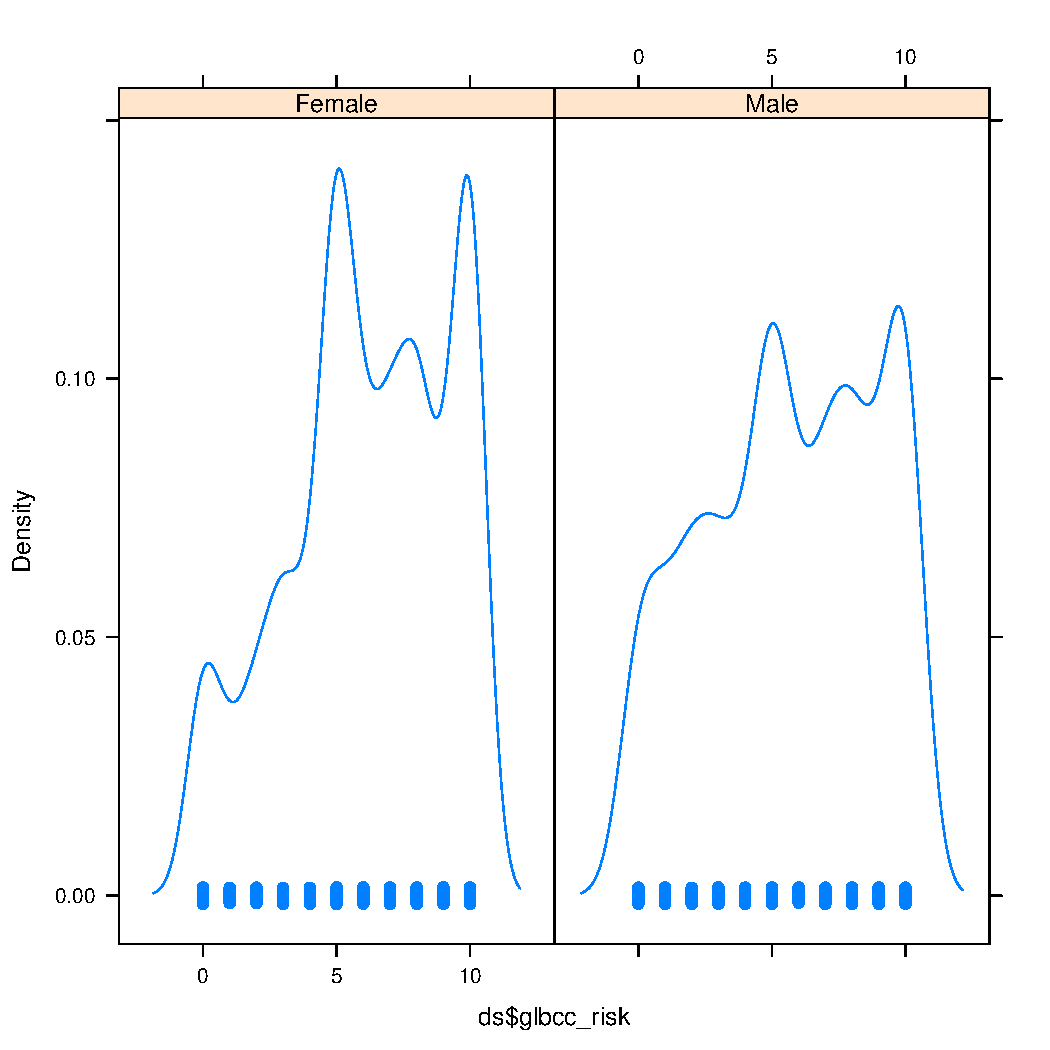
\includegraphics[width=4in, height=4in]{../05_Inference/gendden.pdf}%filename
\caption{Density Plots of Climate Change Risk by Gender}
\end{figure}   

Based on the density plots, it appears that some differences exist between males and females regarding perceived climate change risk. We can also use the \texttt{by} command to see the \texttt{gccrsk} mean of climate change risk for males and females.
\begin{knitrout}
\definecolor{shadecolor}{rgb}{0.969, 0.969, 0.969}\color{fgcolor}\begin{kframe}
\begin{alltt}
\hlkwd{by}\hlstd{(ds}\hlopt{$}\hlstd{glbcc_risk, ds}\hlopt{$}\hlstd{f.gend, mean,} \hlkwc{na.rm}\hlstd{=}\hlnum{TRUE}\hlstd{)}
\end{alltt}
\begin{verbatim}
## ds$f.gend: Female
## [1] 6.134259
## -------------------------------------------------------- 
## ds$f.gend: Male
## [1] 5.670577
\end{verbatim}
\end{kframe}
\end{knitrout}
\begin{knitrout}
\definecolor{shadecolor}{rgb}{0.969, 0.969, 0.969}\color{fgcolor}\begin{kframe}
\begin{verbatim}
## [1] "Female" "Male"
\end{verbatim}
\end{kframe}
\end{knitrout}
Again there appears to be a difference, with females perceiving greater risk on average (6.13) than males (5.67). However we want to know whether these differences are \textbf{statistically significant}. To test for the statistical significance of the difference between groups, we use a $t$-test. 

\subsection{$t$-tests} 

The $t$-test is based in the $t$ distribution. The $t$ distribution, also known as the Student's $t$ distribution, is the probability 
distribution for \textit{sample} estimates. It has similar properties, and is related to, the normal distribution. The normal distribution is
based on a population where $\mu$ and $\sigma^2$ are known, however the $t$ distribution is based on a sample where $\mu$ and $\sigma^2$
are estimated, as the mean $\bar{X}$ and variance $s^2_x$. The mean of the $t$ distribution, like the normal distribution is $0$, but the
variance, $s^2_x$, is conditioned by $n-1$ \textbf{degrees of freedom}(df). Degrees of freedom are the values used to calculate a statistic that are "free" to vary.\footnote{In a difference of means test across two groups, we "use up" one observation when we separate the observations into two groups. Hence the denominator reflects the loss of that used up observation: n-1.} A $t$ distribution approaches the standard normal distribution as the number of degrees of freedom increase.

In brief, we want to know the difference of means between males and females, $d = \bar{X}_m-\bar{X}_f$ and if that difference is statistically
significant. This amounts to a hypothesis test where our working hypothesis, $H_1$, is that males are less likely than females to view climate
change as risky. The null hypothesis, $H_A$, is that there is no difference between males and females regarding the risks associated with climate
change. To test $H_1$ we use the $t$-test which is calculated: 
\begin{equation}
  \label{eq:t}
  t = \frac{\bar{X}_m-\bar{X}_f}{SE_d}
\end{equation}
\noindent Where $SE_d$ is the \textbf{standard error} of the estimated differences between the two groups.  To estimate $SE_d$ we need the SE of the estimated mean for each group. The SE is calculated: 
\begin{equation}
  \label{eq:se}
  SE = \frac{s}{\sqrt{n}}
\end{equation}
\noindent where $s$ is the s.d. of the variable. $H_1$ states that there is a difference between males and females, therefore under $H_1$ it is expected that $t > 0$ since zero is the mean of the $t$ distribution. However, under $H_A$ it is expected that $t = 0$. 

% t-test by hand
We can calculate this in \texttt{R}. First, we calculate the $n$ size for males and females. Then we calculate the SE for males and females. 
\begin{knitrout}
\definecolor{shadecolor}{rgb}{0.969, 0.969, 0.969}\color{fgcolor}\begin{kframe}
\begin{alltt}
\hlstd{n.total} \hlkwb{<-} \hlkwd{length}\hlstd{(ds}\hlopt{$}\hlstd{gender)}
\hlstd{nM} \hlkwb{<-} \hlkwd{sum}\hlstd{(ds}\hlopt{$}\hlstd{gender,} \hlkwc{na.rm}\hlstd{=}\hlnum{TRUE}\hlstd{)}
\hlstd{nF} \hlkwb{<-} \hlstd{n.total}\hlopt{-}\hlstd{nM}
\hlkwd{by}\hlstd{(ds}\hlopt{$}\hlstd{glbcc_risk, ds}\hlopt{$}\hlstd{f.gend, sd,} \hlkwc{na.rm}\hlstd{=}\hlnum{TRUE}\hlstd{)}
\end{alltt}
\begin{verbatim}
## ds$f.gend: Female
## [1] 2.981938
## -------------------------------------------------------- 
## ds$f.gend: Male
## [1] 3.180171
\end{verbatim}
\begin{alltt}
\hlstd{sdM} \hlkwb{<-} \hlnum{2.82}
\hlstd{seM} \hlkwb{<-} \hlnum{2.82}\hlopt{/}\hlstd{(}\hlkwd{sqrt}\hlstd{(nM))}
\hlstd{seM}
\end{alltt}
\begin{verbatim}
## [1] 0.08803907
\end{verbatim}
\begin{alltt}
\hlstd{sdF} \hlkwb{<-} \hlnum{2.35}
\hlstd{seF} \hlkwb{<-} \hlnum{2.35}\hlopt{/}\hlstd{(}\hlkwd{sqrt}\hlstd{(nF))}
\hlstd{seF}
\end{alltt}
\begin{verbatim}
## [1] 0.06025641
\end{verbatim}
\end{kframe}
\end{knitrout}

\noindent Next, we need to calculate the $SE_d$: 
\begin{equation}
  SE_d = \sqrt{SE^2_M+SE^2_F}  
\end{equation}
\begin{knitrout}
\definecolor{shadecolor}{rgb}{0.969, 0.969, 0.969}\color{fgcolor}\begin{kframe}
\begin{alltt}
\hlstd{seD} \hlkwb{<-} \hlkwd{sqrt}\hlstd{(seM}\hlopt{^}\hlnum{2}\hlopt{+}\hlstd{seF}\hlopt{^}\hlnum{2}\hlstd{)}
\hlstd{seD}
\end{alltt}
\begin{verbatim}
## [1] 0.1066851
\end{verbatim}
\end{kframe}
\end{knitrout}

\noindent Finally, we can calculate our $t$-score, and use the \texttt{t.test} function to check. 
\begin{knitrout}
\definecolor{shadecolor}{rgb}{0.969, 0.969, 0.969}\color{fgcolor}\begin{kframe}
\begin{alltt}
\hlkwd{by}\hlstd{(ds}\hlopt{$}\hlstd{glbcc_risk, ds}\hlopt{$}\hlstd{f.gend, mean,} \hlkwc{na.rm}\hlstd{=}\hlnum{TRUE}\hlstd{)}
\end{alltt}
\begin{verbatim}
## ds$f.gend: Female
## [1] 6.134259
## -------------------------------------------------------- 
## ds$f.gend: Male
## [1] 5.670577
\end{verbatim}
\begin{alltt}
\hlstd{meanF} \hlkwb{<-} \hlnum{6.96}
\hlstd{meanM} \hlkwb{<-} \hlnum{6.42}
\hlstd{t} \hlkwb{<-} \hlstd{(meanF}\hlopt{-}\hlstd{meanM)}\hlopt{/}\hlstd{seD}
\hlstd{t}
\end{alltt}
\begin{verbatim}
## [1] 5.061625
\end{verbatim}
\begin{alltt}
\hlkwd{t.test}\hlstd{(ds}\hlopt{$}\hlstd{glbcc_risk}\hlopt{~}\hlstd{ds}\hlopt{$}\hlstd{gender)}
\end{alltt}
\begin{verbatim}
## 
## 	Welch Two Sample t-test
## 
## data:  ds$glbcc_risk by ds$gender
## t = 3.6927, df = 2097.5, p-value = 0.0002275
## alternative hypothesis: true difference in means is not equal to 0
## 95 percent confidence interval:
##  0.2174340 0.7099311
## sample estimates:
## mean in group 0 mean in group 1 
##        6.134259        5.670577
\end{verbatim}
\end{kframe}
\end{knitrout}

The difference in the percieved risk between women and men, we have a $t$-value of 4.6. This result is greater than zero, as expected by $H_1$. In addition, as shown in the \texttt{t.test} output the \textbf{$p$-value}---the probability of obtaining our result if the population difference was $0$---is extremely low at .0002275} (that's the same as 2.275e-04). Therefore, we \textit{reject the null hypothesis} and concluded that there are differences (on average) in the ways that males and females perceive climate change risk.   

\section{Summary}
In this chapter we gained an understanding of inferential statistics, how to use them to place confidence intervals around an estimate, and got an overview of how to use them to test hypotheses. In the next chapter we turn, more formally, to testing hypotheses using crosstabs and by comparing means of different groups.  After that we continue to explore hypothesis testing and model building using regression analysis.
\end{document}
